\documentclass{article}
\usepackage[margin=3cm]{geometry}
\usepackage[utf8]{inputenc}
\usepackage{amsmath}
\usepackage{amssymb}
\usepackage{float}
\usepackage{enumitem}
\usepackage{graphicx}
\usepackage{caption}
\usepackage{subcaption}

\graphicspath{ {Plots/} }

\begin{document}
	\textit{MS-E2134 - Decision making and problem solving}
	\vfill
	{\centering \Huge Assignment 2 \par}
	\vfill
	Christian Segercrantz - 481056 \\
	\par \today
	\pagebreak
	\tableofcontents
	\pagebreak
\section{Simulation}
\subsection{a)}
\begin{figure}[H]
	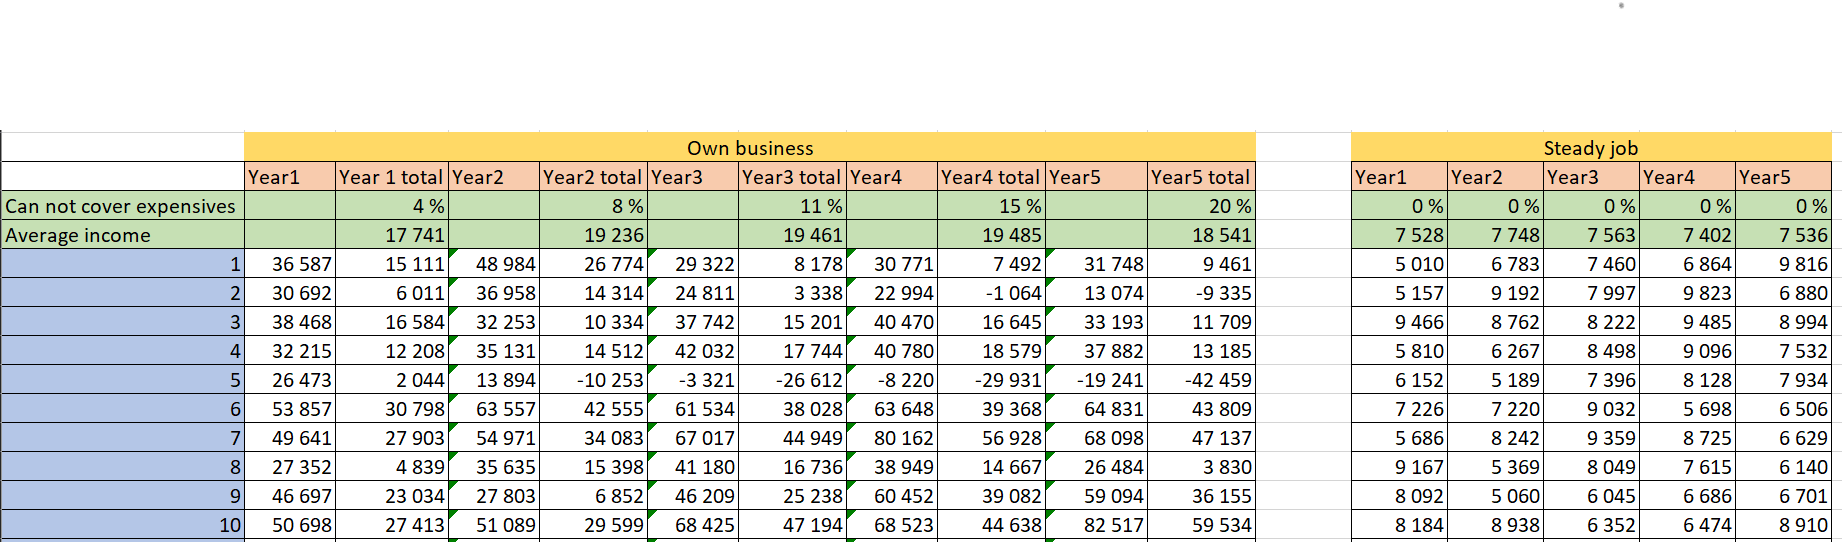
\includegraphics[width=\textwidth]{1a.png}
	\caption{Capion here}
	\label{fig:1a}
\end{figure}

\subsection{b)}

	\begin{table}[h]
		\centering
		\caption{Average cash flow for fives years for both the steady job and own business ventures.}
		\label{tab:1b}
		\begin{tabular}{l|l|l|l|l|l|}
			\cline{2-6}
			& Year 1 & Year 2 & Year 3 & Year 4 & Year 5 \\ \hline
			\multicolumn{1}{|l|}{Steady job}   & 7 528  & 7 748  & 7 563  & 7 402  & 7 536  \\ \hline
			\multicolumn{1}{|l|}{Own business} & 17 741 & 19 236 & 19 461 & 19 485 & 18 541 \\ \hline
		\end{tabular}
	\end{table}
	
	Based on the simulations, it seems that starting a own business venture would for sure be the more lucrative, and better, option. However, an average over 200 replications might give us an overly optimistic outlook.
\subsection{c)}
	We can see the probabilities from Table \ref{tab:1c}. We can see that initially the probability is approximately 5\% and rises to approximately 20\% in year 5. For the steady job, as the maximum of the expenses is less than the constant income, the probability that he is not able to cover his expenses is 0\% for all years.
	\begin{table}[h]
		\centering
		\caption{Probability that Dr. Cuckoo cannot cover his expenses each year for both the steady job and own business ventures.}
		\label{tab:1c}
		\begin{tabular}{l|l|l|l|l|l|}
			\cline{2-6}
			& Year 1 & Year 2 & Year 3 & Year 4 & Year 5 \\ \hline
			\multicolumn{1}{|l|}{Steady job}   & 0 \%   & 0 \%   & 0 \%   & 0 \%   & 0 \%   \\ \hline
			\multicolumn{1}{|l|}{Own business} & 4 \%   & 8 \%   & 11 \%  & 15 \%  & 20 \%  \\ \hline
		\end{tabular}
	\end{table}
\section{Decision trees}
\section{Elicitation of utility functions}
	We start by calculating the different values for the utility functions. We normalize the utility function such that $u(10M)=1$ and $u(-2M)=0$. We can thus calculate:
	\begin{align}
		u(1.5\text{M}) &= 0.5u(10\text{M}) + 0.5u(-2\text{M})\\
		u(1.5\text{M}) &= 0.5 \cdot 1 + 0.5 \cdot 0 \\ 
		u(1.5\text{M})&= 0.5 \\
		u(4\text{M}) &= 0.5u(10\text{M}) + 0.5u(1.5\text{M})\\
		u(4\text{M}) &= 0.5 \cdot 1 + 0.5 \cdot 0.5 \\ 
		u(4\text{M})&= 0.75 \\
		u(0.1\text{M}) &= 0.5u(-2\text{M}) + 0.5u(1.5\text{M})\\
		u(0.1\text{M}) &= 0.5 \cdot 0 + 0.5 \cdot 0.5 \\ 
		u(0.1\text{M})&= 0.25 \\
		u(6\text{M}) &= 0.4u(10\text{M}) + 0.6u(4\text{M})\\
		u(6\text{M}) &= 0.4 \cdot 1 + 0.6 \cdot 0.75\\ 
		u(6\text{M})&= 0.85 \\
	\end{align}
	The plotted utility function can be seen in Figure \ref{fig:3}. As we can see, the function is somewhat concave. According to EUT, Dr. Stoveo is, as he says, risk averse.
	\begin{figure}[H]
		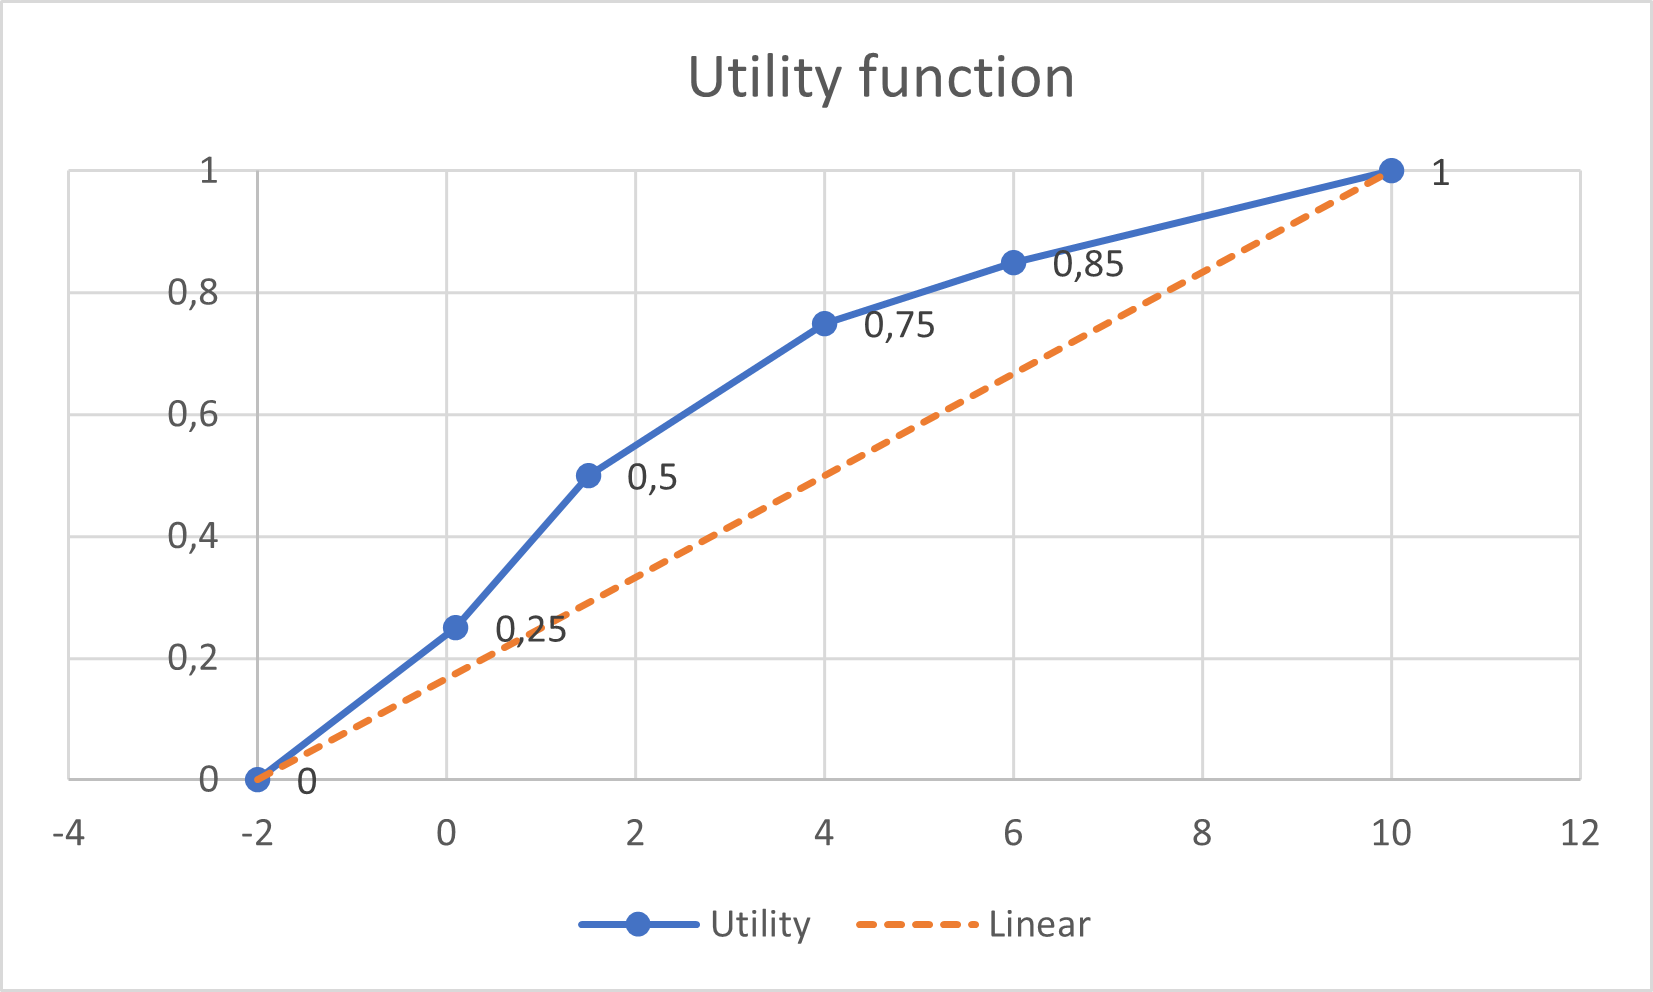
\includegraphics[width=0.9\textwidth]{3.png}
		\caption{The plotted utility function based on Dr. Stoveos choices.}
		\label{fig:3}
	\end{figure}
\end{document}